\begin{figure*}[t]
    \centering
    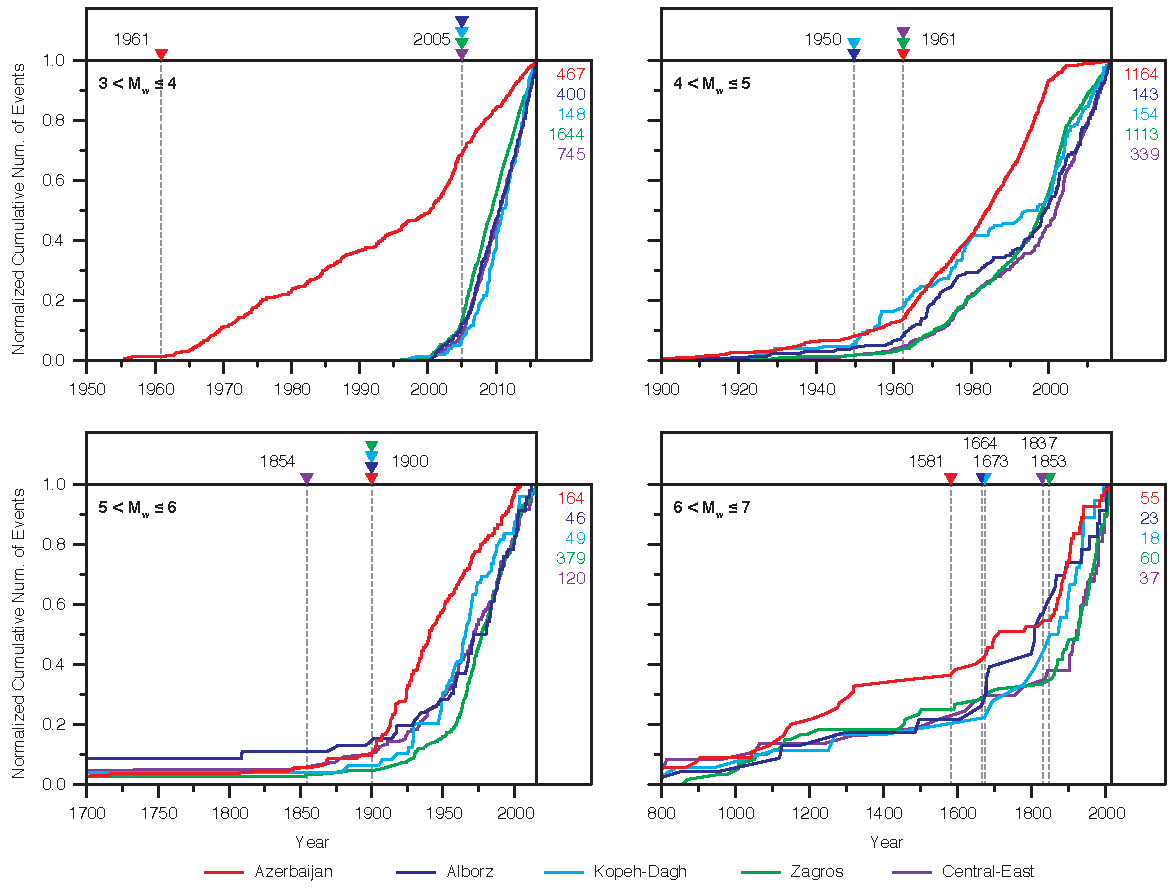
\includegraphics[width=0.8\textwidth]{figures/pdf/figure-05.pdf} 
    \caption{Normalized cumulative number of events and completeness year thresholds for each of the seismic zones considered within the region of interest, and for magnitude intervals of $\Delta M = 1$ between $M_w$ 3 and 6. The year thresholds are indicated by a triangle mark at the top and the vertical dashed lines in the background. Normalization values for each curve are indicated on the right margins and distinguished by color as indicated in the legend.}
    \label{fig:completeness}
\end{figure*}

\subsection{Completeness}

An important aspect of seismic catalogs is their completeness. This characteristic is measured in terms of the year of completeness and the completeness magnitude, which are used as parameters in the seismic analysis process. In simple terms, the year of completeness is the point in time at which catalog data exhibits a steady rate of event occurrence or record accumulation. This point is typically identified for different magnitude ranges. A simple approach used by \citet{Frankel1995} and others is to select the year at which a plot of the cumulative number of events with respect to time becomes (or starts to resemble) a straight line.

On the other hand, The completeness magnitude, denoted as $M_c$, is the minimum magnitude at which the seismic catalog of a region can be considered complete within a certain time period. While the year of completeness can be determined by inspection of the data, the completeness magnitude often requires a numerical analysis of the catalog. A common approach consists on identifying the magnitude associated with the maximum value of the first derivative of the frequency-magnitude curve. This method is widely used and has been implemented in the ZMAP software package for seismic hazard analysis developed by \citet{Wiemer2001}. \citet{Zare2014}, for instance, used this method to identify $M_c$ values for the different regions of the Middle East.

One of the difficulties in determining completeness is the availability of data for a period of time long enough for all magnitude ranges, so that selection of completeness parameters is reliable. In this study, we determined the year of completeness for magnitude ranges 3--4, 4--5, 5--6 and 6--7 by inspection, following the approach used by \citet{Frankel1995}. This is illustrated in Fig.~\ref{fig:completeness}, where we show the normalized cumulative number of events with time for each of the seismic zones and magnitude ranges, and indicate our choice of the completeness year thresholds in each case. For events $M_w>7$, in which case there are no sufficient data to determine a proper threshold, we assumed the catalog to be complete from the earliest time at which there is record of large magnitude earthquakes. 

Admittedly, the choice of the threshold years is highly subjective. We should note then, that in the process of choosing the points indicated in the plots shown in Fig.~\ref{fig:completeness}, we considered additional contributing information such as the history of instrumentation. It is well known, for instance, that the number of recorded earthquakes increased considerably after the first deployment of seismic instruments in the early 1900s, and later with the establishment of the Worldwide Standardized Seismograph Network in 1961. We also compared our choices with the year thresholds reported by \citet{Zare2014}, which we found to be consistently earlier than our preferred years of completeness. In the end, we proceeded with our selection, which leads to a more conservative estimation of hazard.

For the case of the completeness magnitude $M_c$, we adopted the values reported by \citet{Karimiparidari2013}. Our choice the $M_c$ values by \citet{Karimiparidari2013} over those of \citet{Zare2014} is based on the fact that the former distinguishes Azerbaijan and Alborz as individual seismic zones---as we do---as opposed to the approach followed by the latter, in which these two are a single, larger seismic zone. Both the chosen years of completeness and the values of completeness magnitude for each seismic zone and for the uniform model of the entire region of interest are summarized in Table \ref{tab:completeness}.

\begin{table}%[t]
    \centering
    \caption{Year thresholds and magnitude completeness for the seismic zones within the region of interest in this study.}
    \begin{tabular}{@{\hspace{0.2ex}}lccccrc@{\hspace{0.2ex}}}
        \cline{2-7}                                              \\[-1.6ex]
                        & 3--4 & 4--5 & 5--6 & 6--7 & 
                                  \multicolumn{1}{c}{$>7$} &$M_c$\\[0.6ex]
        \hline                                                   \\[-1.6ex]
        Azerbaijan      & 1961 & 1961 & 1900 & 1581 & 1042 & 4.5 \\
        Alborz          & 2005 & 1950 & 1900 & 1664 &--401 & 4.4 \\
        Kopeh Dagh      & 2005 & 1950 & 1900 & 1673 &    9 & 4.5 \\
        Zagros          & 2005 & 1961 & 1900 & 1853 & 1439 & 4.4 \\
        Central-East    & 2005 & 1961 & 1854 & 1837 &  762 & 4.5 \\
        Uniform Model   & 2005 & 1961 & 1900 & 1778 &--401 & 4.5 \\[0.5ex]
        \hline 
    \end{tabular}
    \label{tab:completeness} 
\end{table}


% *********************************************************************************************************************
% OLD STUFF
% *********************************************************************************************************************

% For the smoothed seismicity method, completeness of each magnitude in the catalog is an important factor.  \citet{Frankel1995} plotted the cumulative number of events against time for different regions. He assumes that from the point that the line become linear, the catalog is complete. This approach is similar to the MAXC method of ZMAP software \citep{Wiemer2001}, where the completeness treshold is the maximum value of the first derivative of the frequency-magnitude curve. 

% Using the cumulative frequency-magnitude distribution of \citet{Gutenberg1944} and also frequency magnitude distribution approach in software ZMAP, \citet{Zare2014} reported the catalog completeness for the study regions. 

% World widely large earthquakes were routinely located after increasing number of seismic stations establishment in the early 1900s \citep{Shearer2009}. Up to 1961 these data formed the early instrumental period. In 1961 the Worldwide Standardized Seismograph Network (WWSSN) was stablished. The record of these seismographs considerably improved the seismic catalogs in different part of the world \citep{Shearer2009}. Fig.~\ref{fig:completness_scatter} shows the magnitude distribution of events with respect to the time of occurrence of the events.

% We pick the Mw 0.5 increments in magnitude to be able to compare the results with \citet{Zare2014}. In order to be able to compare the results with \citet{Zare2014} we merge the data of Azerbaijan and Alborz seismic regions.  Fig.~\ref{fig:completness_compare_zare_2014_Az_Al} shows the completeness of catalog for earthquakes with different magnitude range in Azerbaijan-Alborz region. According to this figure, midrange magnitudes ($ 4 < Mw < 6 $) fairly obey the network developments in 1900 and 1961. The completeness thresholds for each magnitude range which are reported by \citet{Zare2014} are shown by dashed green line. 

% In this study we follow the \citet{Frankel1995} approach to determine the completeness of each region. Even though the approach used by \citet{Frankel1995} will lead to the conservative results, we make sure that we don't use a period of time without knowing the complete number of events. Determining the completeness of the catalog is very sensitive to the data. Converting earthquake magnitudes from different scales to moment magnitude obviously has some error. Having broader range of magnitude will help to minimize these sort of error. In this study we consider the magnitude intervals for completeness study as $Mw = 1$. 



